\documentclass[../../main.tex]{subfiles}

\graphicspath{{../../fig/}}
\setcounter{section}{0}

\begin{document}
\chapter{スパースワイヤーグリッドを用いた偏光角較正装置}
SOでは検出器の偏光角較正のために、人工偏光光源としてスパースワイヤーグリッドを用いた偏光角較正装置を使用する。
本章では、スパースワイヤーグリッドの外観を共有した後に偏光角の較正原理について触れ、装置の設計、系統誤差要素について述べる。

\section{偏光信号の生成原理}
金属製のワイヤーが、周囲から来た入射光を反射することを考える。
入射光の波長がワイヤーの直径よりも十分に長い場合、ワイヤー中の自由電子はワイヤーに沿う方向のみに動くと見なすことができ、ワイヤーは自身の軸に沿った偏光状態を持つ光のみを反射する。
このようなワイヤーを望遠鏡の視野に置くと、ワイヤーは周囲の環境から来る熱放射を反射し、ワイヤー軸と同じ方向に偏光した光を望遠鏡に送り込む。
実際には望遠鏡は空も視野に含み、無偏光な大気放射、ワイヤーからの偏光信号の重ね合わせが見える。
\ref{}にて述べた、回転半波長板という光学素子を用いることで無偏光な大気放射を取り除き、ワイヤーからの偏光信号のみを抽出して偏光角較正に用いる。
また、ワイヤー間隔を調整することで実行的な放射温度を調整し、CMB望遠鏡の検出器に入射する光の強度を調整することができる。

\section{偏光角較正の原理}
式\eqref{eq:so-hwp_modulation}において、入射光としてワイヤー由来の偏光角 $\theta_{\mathrm{wire}}$ の直線偏光した光を考える。
$Q_{\mathrm{in}}(t) + iU_{\mathrm{in}}(t) = \exp\qty[2i\theta_{\mathrm{wire}}]$ となるため、
\begin{equation}
    d_{\mathrm{m}, \mathrm{det}}(t) = I_{\mathrm{in}}(t) + \varepsilon\Re\qty[\exp\qty{-i \qty(4\omega_{\mathrm{HWP}}t + 4\chi_0 - 2\theta_{\mathrm{det}} - 2\theta_{\mathrm{wire}})}]
\end{equation}
となる。
ワイヤー由来の光の強度はほとんど時間変化しないため、$I_{\mathrm{in}}(t) \simeq \mathrm{const.}$ とみなせる。
したがって、この変調信号は時系列データとして位相オフセット $4\chi_0 + 2(\theta_{\mathrm{det}} + \theta_{\mathrm{wire}})$ を持った
角振動数 $4\omega_{\mathrm{HWP}}$ の正弦波としてみえる。
理想的な時系列データのイメージを図\ref{fig:}に示す。
これを復調することで、式\eqref{eq:so-hwp_demod}より
\begin{equation}
    d_{\mathrm{d, det}} = \varepsilon\exp\qty[i2\qty(\theta_{\mathrm{wire}} + \theta_{\mathrm{det}})]
\end{equation}
という偏光情報のみを得る。
望遠鏡では光学系により生まれる偽偏光や、環境熱放射が比等方だった場合にはワイヤー角度に対して非等方な強度のワイヤー由来の偏光が観測され得る。
これを取り除くため、さまざまなワイヤーの角度 $\theta_{\mathrm{wire}}$ でこの $d_{\mathrm{d, det}}$ を測定し、複素平面上で円(較正円と呼ぶ)を描く(\ref{fig:})。
光学系による偽偏光は較正円の原点がズレる効果として現れ、環境熱放射の非等方性は較正円を歪ませる効果として現れる。
この較正円を用いて補正を加え、最終的に検出器の偏光角 $\theta_{\mathrm{det}}$ を較正する。
\begin{figure}
    \centering
    \caption[スパースワイヤーグリッドによって生成される偏光信号の時系列データイメージ]{スパースワイヤーグリッドによって生成される偏光信号の時系列データイメージ。}
\end{figure}
\section{較正装置の設計と特徴}
較正円を描くためにはスパースワイヤーグリッドを回転させ、ワイヤーの角度を変化させる必要がある。
また、本装置は望遠鏡の窓の前に設置されるという特性上、CMB観測時にはそれを取り外さなければならない。
先行研究ではこのような回転・切り替え作業を手動にて行ってきたが、それに伴って短期間での再較正が困難であった。
そこで、本装置ではワイヤーの回転と観測・較正の切り替えを自動で行う機構が開発・搭載され、10分程度での較正が実現されている。
本節では、スパースワイヤーグリッド本体の設計に加え、この自動化機構について述べる。
\subsection{スパースワイヤーグリッドの設計}
スパースワイヤーグリッドの外観を図\ref{fig:wiregrid_appearance}に示す。
これは金属製のワイヤーを、入射光よりも十分長い間隔で平行に張ったものであり、ワイヤー軸に沿った偏光を生成する。
SOではアルミニウム製の内径$\SI{790}{mm}$、外径 $\SI{830}{mm}$ の円環に、直径 $\SI{0.1}{mm}$ の
タングステンワイヤーを $\SI{20}{mm}$ 間隔で $39$ 本張り巡らせたものを使用する\cite{swg:murata}。
\begin{figure}[H]
    \centering
    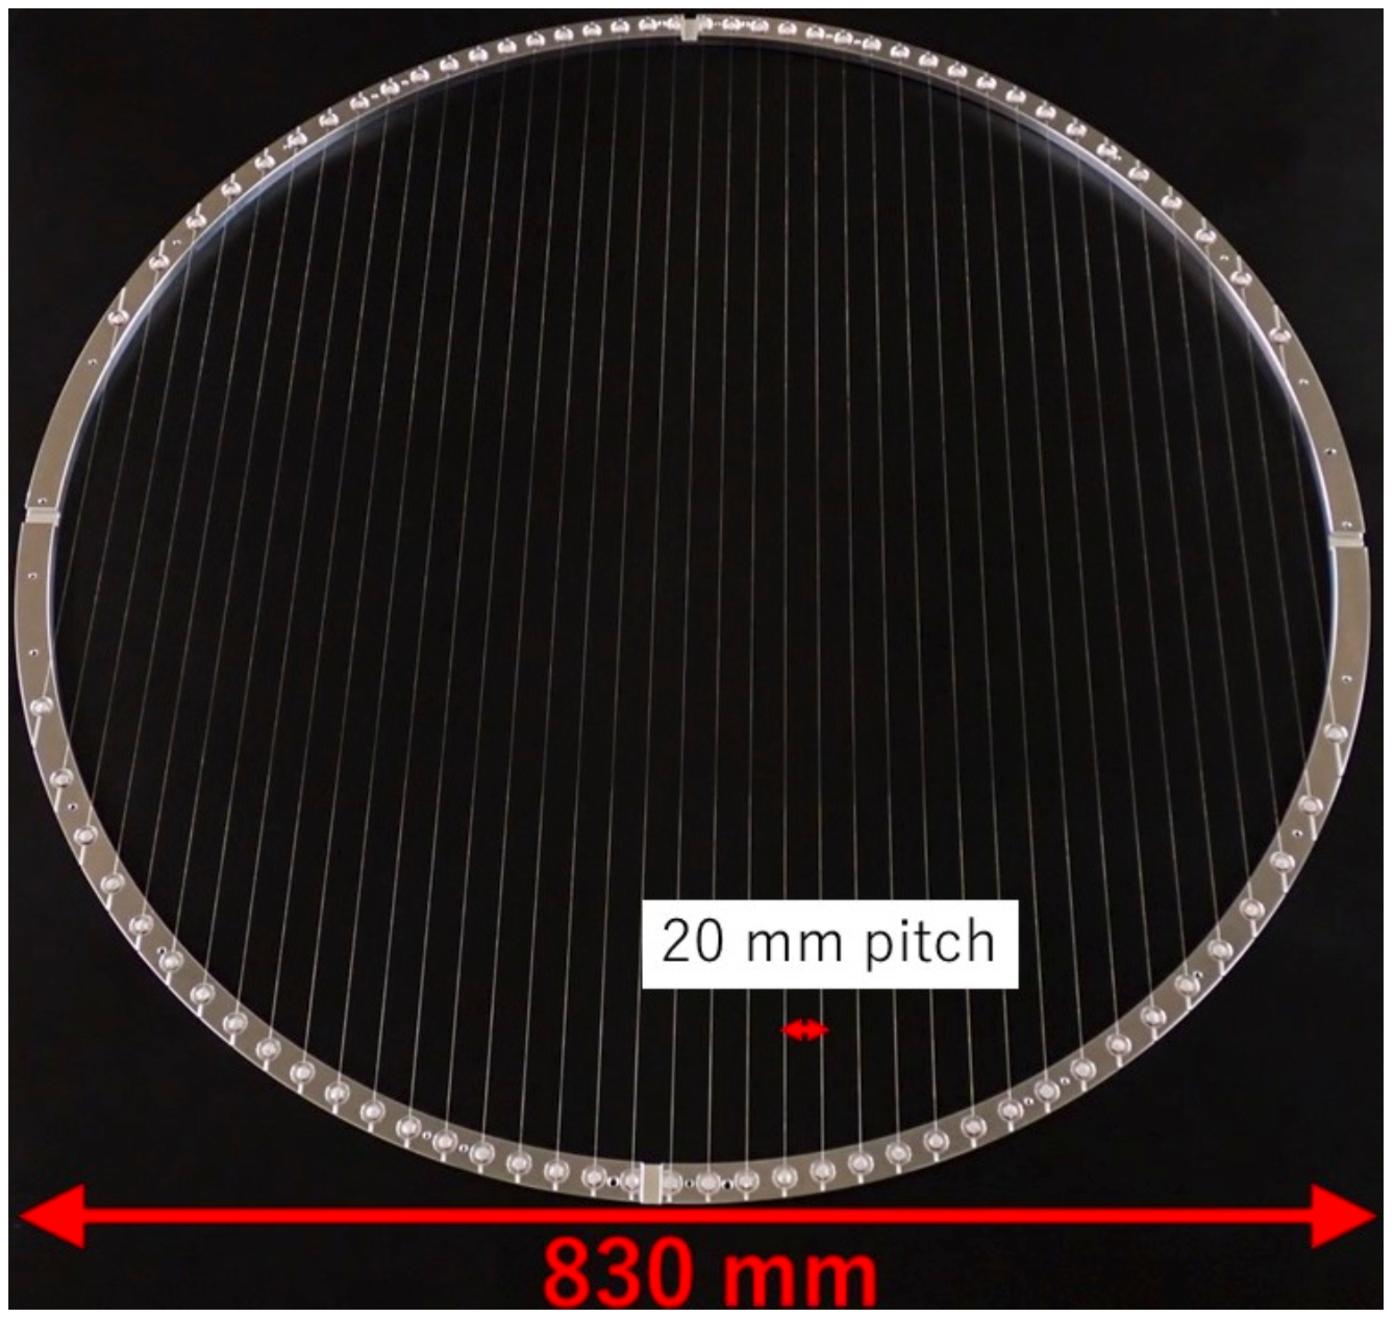
\includegraphics[width=0.5\textwidth]{wiregrid/wiregrid_appearance.pdf}
    \caption[スパースワイヤーグリッド本体の外観]{スパースワイヤーグリッド本体の概観}
    \label{fig:wiregrid_appearance}
\end{figure}
\subsection{回転機構}
Crouzet USA 社製の STANDARD MOTOR 2900 RPM 12V というDCモーターを使用し、スパースワイヤーグリッドを回転させる。
図\ref{fig:rotation_parts}に回転機構の概観を示す。
回転角度は RENISHAW 社製の LM15IC という磁気エンコーダを用いて測定されており、$0.003\tcdegree$ の精度で常にモニターされる。
モニターされた角度を用いてDCモーターへの電流を制御するシステムが開発されており、
これによりスパースワイヤーグリッドを$\order{1\tcdegree}$ の精度で $22.5\tcdegree$ ずつ回転させ、較正円を描く\cite{swg:nakata}。
\begin{figure}[H]
    \centering
    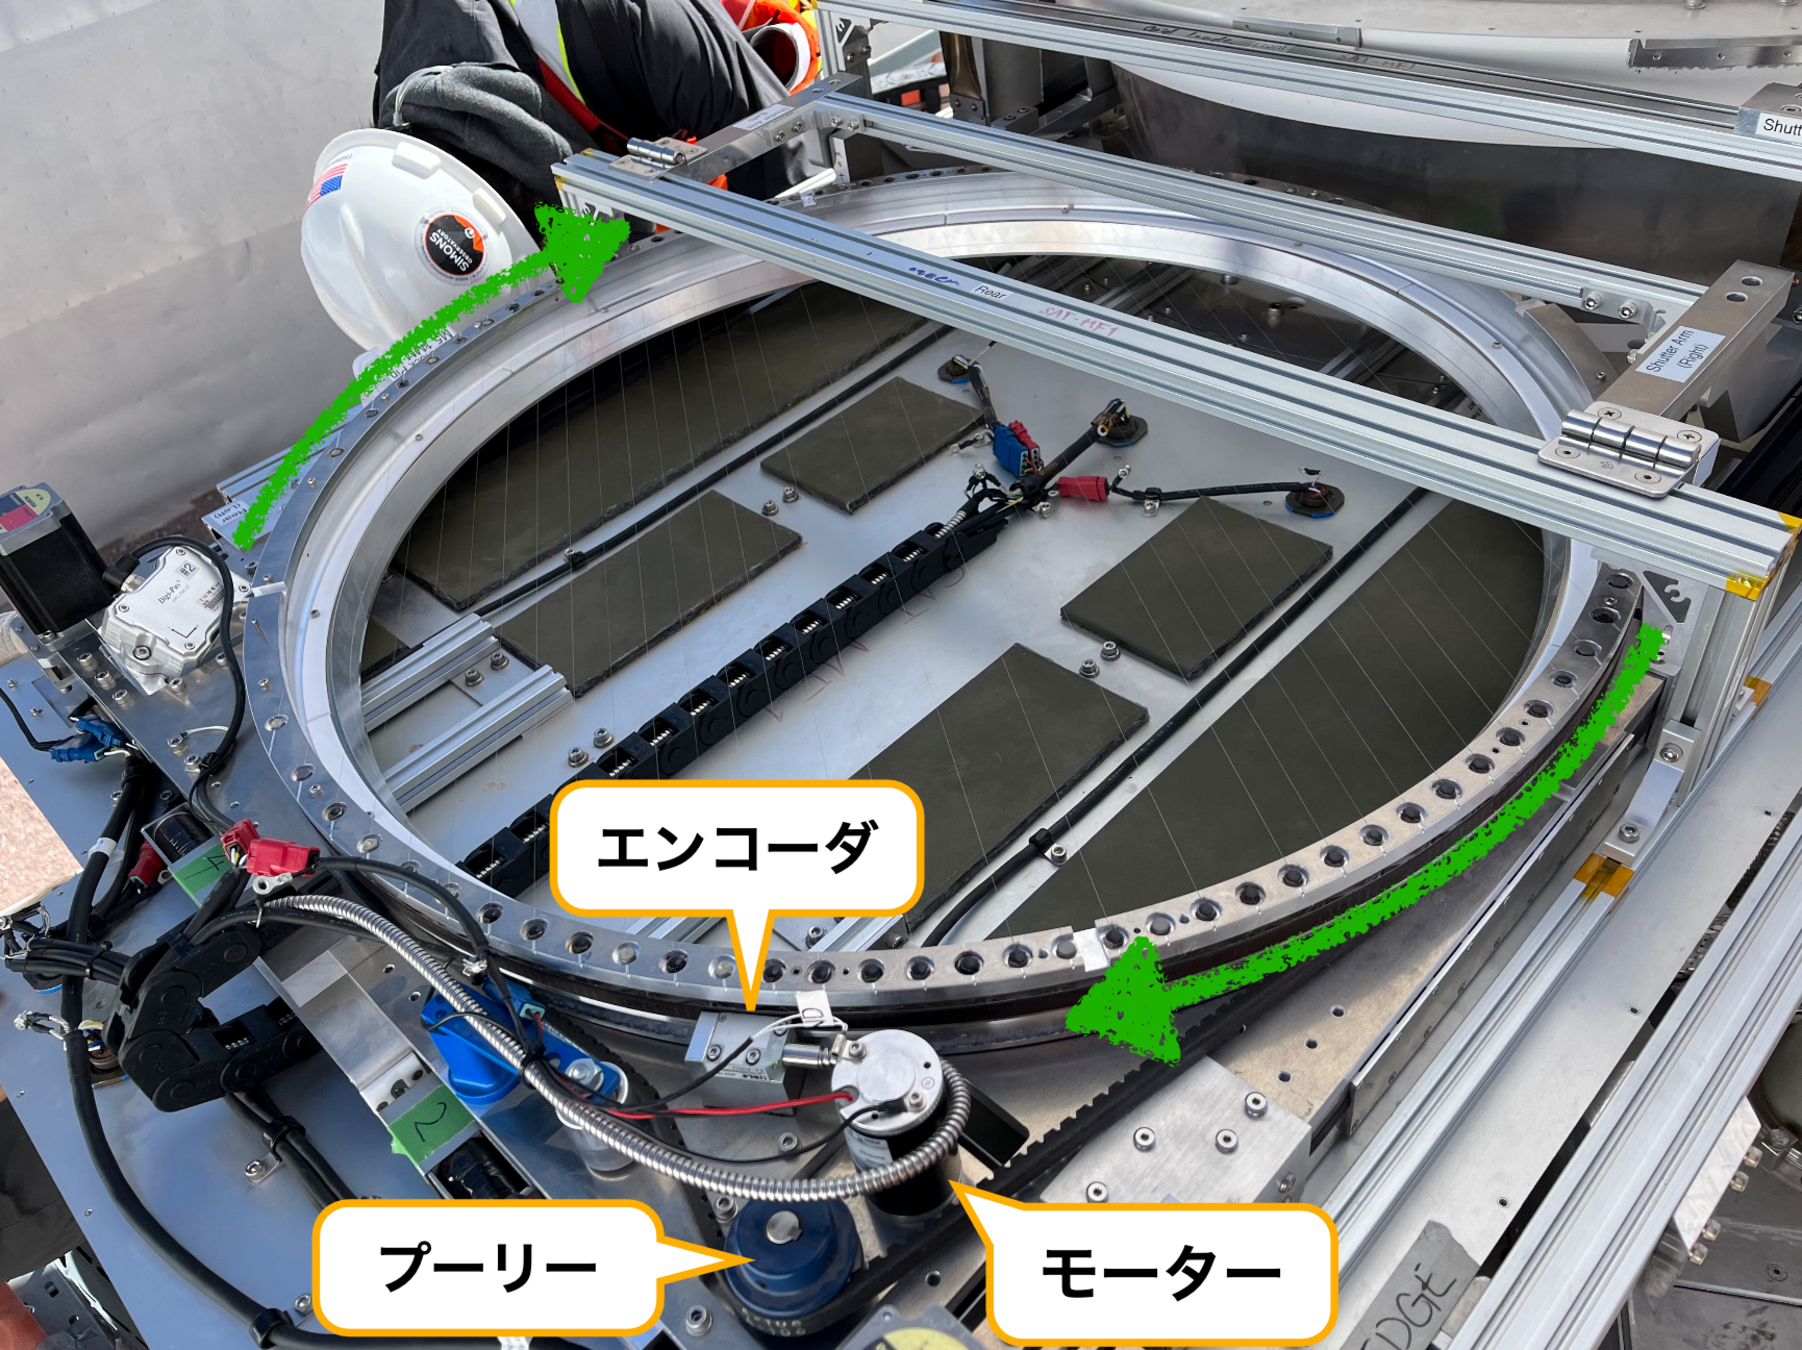
\includegraphics[width=0.8\textwidth]{wiregrid/rotation_parts.pdf}
    \caption{スパースワイヤーグリッドに搭載された回転機構の概観}
    \label{fig:rotation_parts}
\end{figure}
\subsection{切り替え機構}
本較正装置ではCMB観測モードと較正モードの切り替えを2本のアクチュエータによって
スパースワイヤーグリッドを出し入れすることで実現している。
図\ref{}に切り替え機構の概観を示す。
アクチュエータのモーターには Oriental motor 社製の PK269JDA という2相式ステッピングモーターを使用しており、
アクチュエータの両端にあるリミットスイッチによりスパースワイヤーグリッドが端まで移動したことを認識、動作を止める。
本機構によるスパースワイヤーグリッドの出し入れは片道で $90$ 秒程度となっており、CMB観測の時間を無駄にすることなく較正を行うことに貢献している\cite{swg:nakata}。
\begin{figure}
    \centering
    \caption[スパースワイヤーグリッドに搭載された切り替え機構の概観]{スパースワイヤーグリッドに搭載された切り替え機構の概観}
    \label{fig:gridloader}
\end{figure}
\subsection{重力参照計を用いた $\theta_{\mathrm{wire}}$ の測定}
式\eqref{}において、 $\theta_{\mathrm{wire}}$ は天球面上における偏光角である。
エンコーダはスパースワイヤーグリッドが、その平面内において回転したワイヤーの角度を出力するので、
この平面が天球面上のどこに位置しているかを知る必要がある。



\section{系統誤差要素}



\end{document}